% !TeX root = ./main.tex

\documentclass[12pt]{report}
 
%%%%%%%%%%%%%%%%%%%%%%%%%%%%%%%%%%%%%%%%%%%%%%%%%%%%%%%%%%%%%%%%%%%%%%%%%%%%%%%%%%%%%%%
\usepackage[margin=1in]{geometry} 
\usepackage{amsmath,amsthm,amssymb}
\usepackage[utf8]{inputenc}
\usepackage{amsmath}
\usepackage[shortlabels]{enumitem}
\usepackage{mathtools}
\usepackage{amsfonts}
\usepackage{float}
\usepackage{epigraph}
\usepackage{lipsum}
\usepackage{parskip}
\usepackage[spanish]{babel}
\usepackage{tikz}
\usetikzlibrary{babel}
\usepackage{caption}
\usepackage{subcaption}

\usepackage{csquotes}
\usepackage{xcolor}
\usepackage[framemethod=tikz,xcolor=true]{mdframed}
\usepackage[new]{old-arrows}
\usepackage{listings}
%%%%%%%%%%%%%%%%%%%%%%%%%%%%%%%%%%%%%%%%%%%%%%%%%%%%%%%%%%%%%%%%%%%%%%%%%%%%%%%%%%%%%%%

%%%%%%%%%%%%%%%%%%%%%%%%%%%%%%%%%%%%%%%%%%%%%%%%%%%%%%%%%%%%%%%%%%%%%%%%%%%%%%%%%%%%%%%
% mis comandos
\usepackage{personalcommands}
\newtheorem{theorem}{Teorema}[chapter]
\newtheorem{lemma}[theorem]{Lema}
\newtheorem{prop}[theorem]{Proposición}
\newtheorem{coro}[theorem]{Corolario}
\newtheorem{conj}[theorem]{Conjetura}
\newtheorem{ejercicio}{Ejercicio}[section]
\newtheorem*{ejercicio*}{Ejercicio}
\theoremstyle{definition}
\newtheorem{definition}[theorem]{Definición}
\newtheorem{example}[theorem]{Ejemplo}
\theoremstyle{remark}
\newtheorem{remark}[theorem]{Nota}
\newtheorem{notacion}[theorem]{Notación}
%%%%%%%%%%%%%%%%%%%%%%%%%%%%%%%%%%%%%%%%%%%%%%%%%%%%%%%%%%%%%%%%%%%%%%%%%%%%%%%%%%%%%%%
            
%%%%%%%%%%%%%%%%%%%%%%%%%%%%%%%%%%%%%%%%%%%%%%%%%%%%%%%%%%%%%%%%%%%%%%%%%%%%%%%%%%%%%%%
% Titulos
\makeatletter
\@ifundefined{@chapapp}{\def\@chapapp{\chaptername}}{}
\makeatother
\usepackage[Lenny]{fncychap}
\ChTitleVar{\Huge\bfseries}
\setcounter{chapter}{0}
%%%%%%%%%%%%%%%%%%%%%%%%%%%%%%%%%%%%%%%%%%%%%%%%%%%%%%%%%%%%%%%%%%%%%%%%%%%%%%%%%%%%%%%

\definecolor{codegreen}{rgb}{0,0.6,0}
\definecolor{codegray}{rgb}{0.5,0.5,0.5}
\definecolor{codepurple}{HTML}{C42043}
\definecolor{backcolour}{HTML}{F2F2F2}
\definecolor{bookColor}{cmyk}{0,0,0,0.90}  
\color{bookColor}

\lstset{upquote=true}

\lstdefinestyle{mystyle}{
    backgroundcolor=\color{backcolour},   
    commentstyle=\color{codegreen},
    keywordstyle=\color{codepurple},
    numberstyle=\numberstyle,
    stringstyle=\color{codepurple},
    basicstyle=\footnotesize\ttfamily,
    breakatwhitespace=false,
    breaklines=true,
    captionpos=b,
    keepspaces=true,
    numbers=left,
    numbersep=10pt,
    showspaces=false,
    showstringspaces=false,
    showtabs=false,
}
\lstset{style=mystyle}

\newcommand\numberstyle[1]{%
    \footnotesize
    \color{codegray}%
    \ttfamily
    \ifnum#1<10 0\fi#1 |%
}

\begin{document}

\tableofcontents

\chapter{Nivel Interno}

Recordemos que un sistema gestor de bases de datos (SGBD) tiene tres niveles distintos: interno, conceptual y lógico. En este tema nos vamos a centrar en el primero de ellos. El nivel interno está formado, a su vez, por otros dos niveles distintos:
\begin{enumerate}[(a)]
\item Comunicación SO: asociado al sistema operativo donde se ejecute el SGBD.
\item Gestión de la información: asociado el SGBD en sí.
\end{enumerate}

\section{Medidas para evaluar un sistema de archivos}

Al final, la información está almacenada en un disco duro, que tienen sistemas de ficheros asociados que les dan estructura. Hay que compararlos para elegir el más eficiente, para ello, tenemos una serie de parámetros:
\begin{center}
\begin{tabular}{|c|l|}
\hline
Parámetro & Mide...\\
\hline
R & la memoria necesaria para almacenar un registro \\
\hline
T & el tiempo para encontrar un registro arbitrario \\
\hline
$T_F$ & el tiempo para encontrar un registro por clave \\
\hline
$T_W$ & el tiempo para escribir un registro cuando ya se tiene su posición \\
\hline
$T_N$ & el tiempo para encontrar el siguiente registro a uno dado \\
\hline
$T_I$ & el tiempo necesario para insertar un registro \\
\hline
$T_U$ & el tiempo necesario para actuar un registro \\
\hline
$T_X$ & el tiempo necesario para leer el archivo \\
\hline
$T_Y$ & el tiempo necesario para reorganizar el archivo \\
\hline
\end{tabular}
\end{center}
\section{Registros y bloques}

Un SGBD almacena la información en tablas. La estructura de las tablas vienen determinadas por las columnas. La información de una tabla se almacena en filas. EL SGBD provee de una serie de tipos de datos para las columnas de una tabla (numéricos, enteros, etc). 

Los ficheros en los que se almacenan las tablas de una base de datos se componen de un conjunto de bloques, que a su vez se componen de un conjunto de registros, que a su vez están compuestos por campos, y en cada campo se almacena un valor.

Los registros, según su longitud ($R$), pueden clasificarse en:
\begin{enumerate}[(a)]
\item Longitud fija: todos los campos tienen longitud fija conocida a priori. Si denotamos por $V_i$ a la longitud del campo $i-$ésimo, entonces la longitud del registro es:
\[
R=\sum_iV_i
\]
\item Longitud variable: hay por lo menos un campo del registro que tiene longitud variable. Con la siguiente notación
\begin{enumerate}
\item $A$: longitud media de los nombres de atributo.
\item $V$: longitud media de los valores de atributo.
\item $a'$: número medio de atributos.
\item $s$: número de separadores por atributo.
\end{enumerate}
tenemos que la longitud del registro es:
\begin{equation}\label{eq:1}
R=a'(A+V+s)
\end{equation}
\end{enumerate}

\begin{example}
Calcular la longitud del siguiente registro de longitud variable:
\begin{center}
\begin{tabular}{|c|c|c|c|c|}
\hline
Factura=325; & Linea=1; & Concepto=Análisis; & Cant=1; & Precio=300; \\
\hline
\end{tabular}
\end{center}
\[
\left.
\begin{array}{c}
A=(7+5+8+4+6)/5=6 \\
V=(2+2+8+2+6)/5=4 \\
s=2
\end{array}
\right\} \Rightarrow R=a'(6+4+2)=12a'
\]
\end{example}

Los \textbf{bloques} son las unidades de transferencia de información del disco a la memoria o viceversa (aunque en memoria se denominan \textit{buffers}). El tamaño del bloque es fijo para toda la base de datos y es múltiplo del tamaño del bloque físico del SO (por eficiencia).

Según su estructura, los bloques se pueden clasificar en:
\begin{enumerate}[(a)]
\item Estructura homogénea: todos los registros tienen la misma estructura, es decir, todos los registros son del mismo tipo y tienen el mismo número de campos.
\item Estructura heterogénea: los registros tienen distinta estructura (los registros tienen distinta longitud). Para usar este tipo, también necesitamos almacenar información sobre la propia estructura del registro.
\end{enumerate}

La relación entre los registros en disco, los bloques del SO y los bloques del SGBD es:
\[
\text{Registro disco} \leftrightarrows \text{Bloque SO} \leftrightarrows \text{Bloque SGBD}
\]

LLamamos \textbf{factor de bloqueo} ($Bfr$), al número de registros que caben en un bloque y depende del tamaño del mismo bloque, $B$, y del tamaño de los registros, $R$. Este valor puede ser fijado a priori por el administrador del SGBD. Siempre incluye una cabecera \textbf{C}, con información útil para el sistema (referencias, fecha de actualización, etc), que tiene que restarse a $B$.

Denominamos \textbf{bloqueo} a la forma en la que se ajustan los registros a un bloque. Hay dos tipos de bloqueo:

\begin{enumerate}[(a)]
\item Fijo o entero: se rellena el bloque con tantos registros como sea posible.
\begin{enumerate}
\item Registro longitud fija:
\[
Bfr=\left\lfloor\frac{B-C}{R}\right\rfloor
\]
\item Registro de longitud variable:
\[
Bfr=\left\lfloor\frac{B-C}{R+M}\right\rfloor
\]
$M$ es el tamaño de las marcas de separación, ya que al ser de longitud variable, las necesitamos para diferenciar entre los registros.
\end{enumerate}
En ambos se redondea hacia abajo ya que si no cabe un registro entero, no podemos guardar una fracción de él.
\item Partido o desencadenado: se escriben registros en un bloque hasta que no quede espacio. Cuando vayamos a insertar el último registro, puede caber entero o partirse en dos partes, cada una en un bloque distinto. Debido a eso, es necesaria la existencia de una referencia del bloque conteniendo el primer trozo, al bloque conteniendo el otro.
\begin{enumerate}
\item Registro longitud fija:
\[
Bfr=\left\lfloor\frac{B-C-P}{R}\right\rfloor
\]
\item Registro de longitud variable:
\[
Bfr=\left\lfloor\frac{B-C-P}{R+M}\right\rfloor
\]
\end{enumerate}
$P$ es el tamaño del puntero al siguiente bloque.
\end{enumerate}

Llamamos \textbf{espacio desperdiciado (W)} al espacio que se pierde en marcas, referencias, espacio en el que no cabe un registro,  etc.
\begin{enumerate}[(a)]
\item Bloqueo partido con registros de longitud variable:
\[
W=\frac{(P+Bfr \cdot M)}{Bfr}=\frac{P}{Bfr}+M
\]
Esa fórmula se puede ver como el porcentaje de espacio del bloque que no es dedicado a almacenar registros. Como es bloque partido, necesitamos un puntero $P$ al siguiente bloque, y como son registros de longitud variable, necesitamos un separador por \textit{cada} registro que almacenamos en ese bloque, es decir, usamos $Bfr\cdot M$ espacio para separadores.
\end{enumerate}

Una vez sabemos medir cuánto espacio se desperdicia en un bloque, podemos saber más o menos que bloqueo es más eficiente teniendo en cuenta el tamaño de los registros:
\begin{enumerate}[(a)]
\item El bloqueo fijo es más eficiente para registros pequeños.
\item El bloqueo partido es más eficiente para registros grandes.
\end{enumerate}

\section{Organización de archivos y métodos de acceso}

\subsection{Archivo Secuencial Físico (ASF)}

En este tipo de archivo suponemos que los registros tienen estructura y longitud variable, es decir, necesitamos \textit{dos} separadores: el primero para separar los campos dentro de un registro y el otro para separar el nombre el campo de su valor. Por ejemplo:
\begin{center}
\begin{tabular}{|c|c|c|c|c|}
\hline
Factura=325; & Linea=1; & Concepto=Análisis; & Cant=1; & Precio=300; \\
\hline
\end{tabular}
\end{center}
\subsubsection{Tamaño de registro}
Si recordamos la expresión \eqref{eq:1}, tenemos que: (porque $s=2$):
\[
R=a'(A+V+2)
\]
\subsubsection{Recuperación de un registro}
\begin{equation}\label{eq:2}
T_F=\sum_{i=1}^n\frac{i}{n}T=\frac{n+1}{2}T\approx\frac{n}{2}T
\end{equation}
\subsubsection{Siguiente registro (por clave)}
\[
T_N=T_F
\]
Como es por clave, el siguiente registro no tiene porqué estar justo después del que tenemos, por lo que hay buscarlo entero de nuevo.
\subsubsection{Inserción de registro}
\[
T_I=T_W
\]
Simplemente hay que abrir el archivo, ir al final e insertarlo.
\subsubsection{Actualización de registro}
Hay que distinguir dos casos:
\begin{enumerate}[(a)]
\item Si el tamaño del registro no cambia, lo único que hay que hacer es encontrarlo y sustituir el nuevo valor:
\[
T_U=T_F+T_W
\]
\item Si el tamaño del registro cambia, entonces primero tenemos que encontrar el registro ($T_F$), marcarlo como inválido ($T_W$) e insertarlo al final ($T_I$):
\[
T_U=T_F+T_W+T_I
\]
\end{enumerate}
\subsubsection{Lectura de fichero}
Hay que distinguir dos casos en función de si queremos que el resultado esté ordenado:
\begin{enumerate}[(a)]
\item Independientemente del contenido del registro: como están seguidos, simplemente hay que leerlos todos:
\[
T_X=nT
\]
\item Lectura ordenada según el valor de un atributo: hay leer el primero, buscar el siguiente, leerlo, buscar el siguiente, es decir: (ojo, al buscarlo ya lo has leído):
\[
T_X=nT_F
\]
\end{enumerate}
\subsubsection{Reorganización del fichero}
Llamemos $O$ al número de registros añadidos y $d$ al número de registros que hay marcados para borrar. Para reorganizarlo, primero debemos leer todos los registros que había antes más los añadios ($n+O$, en $n$, van incluidos también los que hay marcados para borrar). Después, hay que escribirlos todos otra vez, excepto los marcados para borrar. Importante, no consideramos ningún orden, por lo que no hay que tener en cuenta ningún tiempo de ordenación. Además, como lo insertamos en un archivo totalmente nuevo, los podemos escribir directamente $(T_W)$.
\[
T_Y=(n+O)T+(n+O-d)T_W
\]
\subsection{Archivo Secuencial Lógico (ASL)}

En este tipo de archivo, los registros se encuentran ordenados por una \textbf{clave física}, que puede tener uno o varios campos. Además, los registros los consideramos de longitud fija, es decir, tienen los mismos campos y aparecen en el mismo orden. La estructura de los registros se incluye en la cabecera del fichero. Este tipo de registros son muy útiles para hacer estrategias tipo \textit{merge}.

Como los registros están ordenados por una clave, tenemos que insertalos necesariamente en alguna parte del interior del archivo (no al final, en la mayoría de los casos). Esto es terriblemente costoso porque tendríamos que mover todos los registros existentes un lugar hacia abajo para insertar el nuevo registro. Por esta razón, se usa una \textbf{zona de desbordamiento} no ordenada, de tipo ASF. Cuando esta zona de desbordamiento crece, tenemos que reconstruir el fichero haciendo un merge del original con este y reescribiéndolo.

\subsubsection{Tamaño de registro}

Como tienen estructura y longitud fija, simplemente tenemos que considerar lo que ocupa el valor de cada registro (porque la cabecera solo aparece al principio y despreciamos su tamaño):
\[
R=\sum_{i}V_i
\]

\subsubsection{Recuperación de un registro}
Dos casos:
\begin{enumerate}[(a)]
\item Si el valor de búsqueda no es clave, entonces no podemos aprovechar la única ventaja que nos da la estructura de ASL, es decir, sería igual que el ASF \eqref{eq:2}:
\[
T_F=\frac{n}{2}T
\]
\item Si además de no ser clave, hay registros en la zona de desbordamiento, hay que buscarlo en la zona de desbordamiento, es decir, buscarlo en dos ASF de tamaño $n$ y $O$ ($O$ es el tamaño de la zona de desbordamiento):
\[
T_F=\frac{n}{2}T+\frac{O}{2}T
\] 
\item Si el valor de búsqueda es clave, entonces la eficiencia dependerá del algoritmo de búsqueda que usemos. En el mejor de los casos:
\[
T_F\approx \log_2(n)T
\]
\end{enumerate}
\subsubsection{Siguiente registro (por clave)}
Hay que tener en cuenta donde se encuentra el siguiente registro:
\begin{enumerate}[(a)]
\item Si el siguiente valor de clave está en el propio fichero, entonces va a estar justo después del registro que tenemos porque los valores están ordenados, entonces solo tenemos que leerlo:
\[
T_N=T
\]
\item Si el siguiente valor de clave está en la zona de desbordamiento, entonces leemos nuestro registro más todos los de la zona de desbordamiento para buscarlo:
\[
T_N=T+OT
\]
\end{enumerate}
\subsubsection{Inserción de registro}
Como el archivo está ordenado, la inserción es más complicada. Primero tenemos que buscar el sitio que le corresponde al registro, escribirlo y leer y reescribir todos los que haya después de ese:
\[
T_I=T_F+T_W+\frac{n}{2}T+\frac{n}{2}T_W
\]
Si la inserción es de varios registros, es más eficiente insertarlos en el zona de desbordamiento directamente:
\[
T_I=T_W
\]
Pero como después, en algún punto, habrá que insertarlos en el fichero maestro:
\[
T_I=\frac{T_Y}{O}
\]
\textit{esta formula no la entiendo muy bien}
\subsubsection{Actualización de registro}
Hay que distinguir dos casos dependiendo de si se cambia el valor de la clave o no:
\begin{enumerate}[(a)]
\item Si no se cambia el valor de la clave, entonces simplemente hay que encontrarlo y escribir los nuevos valores:
\[
T_U=T_F+T_W
\]
\item Si se cambia el valor de la clave, entonces hay que encontrarlo, marcarlo como inválido, e insertarlo:
\[
T_U=T_F+T_W+T_I
\]
\end{enumerate}
\subsubsection{Lectura de fichero}
\begin{enumerate}[(a)]
\item Si sólo se usa archivo maestro:
\[
T_X=nT
\]
\item Si se usa un fichero de desbordamiento, primero hay que ordenar ese fichero ($T_C(O)$) y después leer ambos ficheros usando $merge$ ($(n+O)T$):
\[
T_X=T_C(O)+(n+O)T
\]
\end{enumerate}
\subsubsection{Reorganización del fichero}
La reorganización de un ASL es muy fácil: consiste en leer el fichero en merge, y reescribir los registros eliminando los borrados:
\[
T_Y=T_X+(n+O-d)T_W=T_C(O)+(n+O)T+(n+O-d)T_W
\]
Importante, si no hay zona de desbordamiento no tiene sentido reorganizar el fichero porque ya está ordenado de por sí.
\subsection{Archivo Secuencial Indexado (denso) (ASI)}

Este tipo de archivo acelera el acceso por clave. Se busca el valor de clave en el \textbf{índice} y éste irá acompañado de una posición en el fichero. Si la posición a la que apunta el índice es un registro, entonces se llama \textbf{índice denso}, si apunta a otro índice, se llama \textbf{índice no denso}.

La estructura de este fichero usa ASLs, descritos en la sección anterior. Manejamos dos ficheros:
\begin{enumerate}[(a)]
\item Un fichero de datos: de tipo ASL con una posible área de desbordamiento (pero que se gestiona de forma distinta al ASL).
\item Un fichero de índice: otro ASL con registros de longitud fija (y estructura uniforme) que contiene valor de clave y dirección del fichero de datos.
\end{enumerate}

\subsubsection{Tamaño de registro}
Al igual que en el ASL, los registros son de longitud fija y estructura uniforme, luego hay que sumar las longitudes de cada atributo. Peo también hay que tener en cuenta el tamaño del índice, que está formado por la clave ($V_K$) y el puntero al registro ($P$):
\[
R=\sum_iV_i + (V_K+P)
\]
\subsubsection{Recuperación de un registro}
La recuperación es muy sencilla, buscar el índice y leer el registro:
\[
T_F=\log_2(n)T+T
\]
\subsubsection{Siguiente registro (por clave)}
Como los índices sí están ordenados, simplemente hay que leer el siguiente índice y luego leer el registro al que apunta su puntero, es decir, dos lecturas sólo:
\[
T_N=T+T=2T
\]
\subsubsection{Inserción de registro}

\begin{enumerate}[(a)]
\item Si el fichero maestro \textbf{no} tiene área de desbordamiento, entonces hay que insertar los registros en el fichero maestro ($T_{I_1}$) además de insertar el registro correspondiente al índice ($T_{I_2}$). Como los dos archivos son ASL, el tiempo de inserción es el mismo que antes:
\[
T_{I_1}=T_{I_2}=T_F+T_W+\frac{n}{2}T+\frac{n}{2}T_W
\]
Como hay que hacer las dos siempre, el tiempo total es la suma de los dos:
\[
T_I=T_{I_1}+T_{I_2}
\]
\item Si el fichero \textbf{sí} tiene zona de desbordamiento, entonces simplemente hay que escribir el registro en ese archivo ($T_W$) e insertar el índice en el archivo de índices, que sigue siendo un ASL, luego:
\[
T_I=T_W+T_{I_2}
\]
\end{enumerate}
\subsubsection{Actualización de registro}

\begin{itemize}[(a)]
\item Si no se cambia el valor de la clave, simplemente hay que entrar el registro a modificar y escribir la modificación.
\[
T_U=T_F+T_W
\]
\item Si se cambia el valor de la clave: hay que buscar el registro que queremos cambiar y marcarlo como inválido ($T_F+T_F$). También hay buscar el índice de ese registro y marcarlo como borrado (el otro $T_F+T_W$). Ahora ya solo hay que insertarlo.
\[
T_U=2(T_F+T_W)+T_{I_1}+T_{I_2}
\]
\end{itemize}

\subsubsection{Lectura de fichero}
\begin{itemize}[(a)]
\item Por índice principal: 
\[
T_X=nT
\]
\item Por índice secundario:
\[
T_X=nT+nT=2nT
\]
\item Por índice secundario y con zona de desbordamiento:
\[
T_X=(n+O)T+nT+OT=2(n+O)T
\]
\end{itemize}
\textit{ver duda profe}
\subsubsection{Reorganización del fichero}

Hay que reordenar los ficheros, pero solo el de desbordamiento, porque el de datos es un ASL luego ya está ordenado. Luego hay que ler la zona de desbordamiento ($OT$), ordenarla ($T_C(O)$), y leer el de datos ($nT)$ haciendo merge entre los dos. Una vez hecho esto, hay que escribir los nuevos datos con sus respectivos índices sin tener en cuenta los borrados($(n+O-d)T_W+(n+O-d)T_W$):
\[
T_Y=T_C(O)+(n+O)T+(n+O-d)T_W+(n+O-d)T_W
\]

\subsection{Archivo Secuencial Indexado (no denso) (ASI)}

Cuando los índices densos alcanzan un tamaño tan grande que no cabe en memoria, es necesario crear índices \textbf{no densos}, es decir, índices que apuntes a \textbf{páginas} de registros. El fichero de índices contendrá tantos índices como páginas tenga el fichero de datos.
\[
\frac{n}{Bfr}
\]
\textit{duda profe}

¿Cómo se busca en un registro no denso? Se selecciona en el índice la clave inmediatamente inferior a la buscada. Se carga el bloque del maestro y ahí se busca secuencialmente. Si no está, hay que acceder al mestro (esto en un denso no era necesario).

Algunas características:
\begin{enumerate}[(a)]
\item En cada página del maestro se suele dejar un espacio para nuevos registros.
\item En maestros con fichero de desbordamiento, cada registro tiene un enlace al siguiente en el fichero de desbordamiento. En una página, hay un enlace a registro de desbordamiento (si la página está completa). En el fichero de desbordamiento, un registro puede tener enlace al siguiente.
\end{enumerate}

\subsection{ASI multinivel}

Solo son efectivos cuando los archivos son grandes y/o los registros son grandes. Si el índice es grande, puede indexarse también. A esto se le llama \textbf{índice multinivel}.

El tamaño de una página del índice viene dado por:
\[
y=\left\lfloor\frac{B-C}{V+P}\right\rfloor
\]
donde $B$ es el tamaño del bloque, $C$ es la cabecera, $V$ el tamaño del valor del índice y $P$ el puntero al siguiente índice.

Si es de $m$ niveles, todos los niveles son no densos. La estructura es de árbol. Al primer nivel se le llama \textit{raíz}. El nivel 1 es el más cercano al fichero maestro.

En general, el fichero maestro tiene desbordamiento:
\[
r=P+\sum_iV_i
\]
\textit{duda profe}

El índice de primer nivel tiene una entrada por bloque del maestro, luego el número de entradas es:
\[
i_1=\left\lceil\frac{n}{Bfr}\right\rceil
\]
El redondeo es hacia arriba porque necesitamos un índice de bloque para todos los registros, incluso si solo hay un registro en ese bloque.

Los niveles superiores tienen su propio tamaño de bloque $B$ y tamaño de página del índice $y$. Luego su número de entradas es:
\[
y_k=\left\lceil\frac{y_{k-1}}{y}\right\rceil
\]
Y número de bloques:
\[
b_k=\left\lceil\frac{i_k}{y}\right\rceil=i_{k+1}
\]
Claramente, el espacio necesario para índices, es la suma de todos los bloques por el espacio que ocupa un bloque:
\[
I=(b_1+\cdots+b_m)B
\]
Y el \textbf{espacio medio} necesario por registro se calcula como una media del tamaño de todos los índices entre cada registro ($I/n$), 
\textit{duda profe que tiene que ver con la r anterior}
\[
R=r+\frac{O}{n}r+\frac{I}{n}
\]

\subsubsection{Recuperación de un registro}

\[
T_F=T_M+(m-1)T_{F_i}+T_F'
\]
\subsection{Archivo de Acceso Directo (AAD)}

\subsubsection{Tamaño de registro}
\subsubsection{Recuperación de un registro}
\subsubsection{Siguiente registro (por clave)}
\subsubsection{Inserción de registro}
\subsubsection{Actualización de registro}
\subsubsection{Lectura de fichero}
\subsubsection{Reorganización del fichero}


\section{Evaluación del sistema}
\chapter{Optimización de consultas}

Organizar más adecuadamente la información a nivel físico no es lo único por hacer cuando se optimiza el funcionamiento de una BD. Las operaciones más ejecutadas en una base de datos son las consultas, y estas pueden ser optimizadas (transformadas antes de su ejecución para que se ejecuten de la forma más eficiente posible -en tiempo y espacio-), pero este proceso también gasta tiempo.

El \textbf{optimizador} es el módulo del SGBD que efectúa modificaciones en la consulta para obtener los datos consultados de la forma más eficiente tratando de reducir:
\begin{enumerate}[(a)]
\item El tiempo de evaluación o
\item El tiempo de respuesta
\end{enumerate}
El coste minimizable se base en dos costes diferentes:
\begin{enumerate}[(a)]
\item Coste de acceso a almacenamiento secundario
\item Coste computacional (basado en el número de comparaciones)
\end{enumerate}
\medskip
\begin{example}
Supongamos que tengamos la siguiente tabla en la base de datos:
\begin{itemize}
\item Alumno (DNI, nombre, fec\_nac, ciudad, direccion, tlfno, beca)
\item Asignatura (codigo, nombre, creditos, caracter, curso)
\item Matricula (codigo, DNI, calificacion)
\end{itemize}

Consulta que queremos optimizar:
\begin{lstlisting}[ language=SQL,
                    deletekeywords={IDENTITY},
                    deletekeywords={[2]INT},
                    morekeywords={clustered},
                    framesep=8pt,
                    xleftmargin=40pt,
                    framexleftmargin=40pt,
                    frame=tb,
                    framerule=0pt ]
  SELECT alumno.nombre FROM alumno, matricula 
  WHERE alumno.DNI = matricula.DNI 
  AND beca = "N" 
  AND calificacion LIKE "SOBRESALIENTE HONOR";
\end{lstlisting}

Suponiendo que la eficiencia de la ordenación es $O(n\log_2(n))$y la tabla cumple:
\begin{center}
\begin{tabular}{|c|c|c|c|c|c|}
\hline 
Relación & NTuplas & Bfr & Cond1 & Cond2 & Cond1 y Cond2 \\ 
\hline 
Alumno & 500 & 5 & 100 &  & 15 \\ 
\hline 
Matricula & 5000 & 10 & & 120 &  \\ 
\hline 
\end{tabular}
\end{center}

\begin{enumerate}
\item Primera alternativa: hacer primero el producto cartesiano, es decir, tendríamos $500\cdot5000=2500000$ registros. Teniendo en cuenta el $Bfr$ de cada una de las tablas, tendríamos $(500/5)\cdot(5000/10)=50000$ bloques de E/S. Las tendrá que escribir a disco ($Bfr=3$), luego habrá 833334 bloques.

Después hacemos la selección, es decir, tenemos que leer todos los bloques y escribir los 15 registros resultantes (en 5 bloques).

Por último, tenemos que realizar la proyección, es decir, leer los 5 bloques y escribir los 15 nombres, que caben en un bloque. En total:
\[
nºbloques=50000+833334\cdot 2+5+5+1=1716679 \text{ bloques }
\]
Conclusión: demasiado costoso.
\item Segunda alternativa: ordenamos por matrícula, que como tiene 5000 registros y su $Bfr$ es 10, tendríamos que leer 500 bloques. Como la eficiencia es $n\log_2(n)$, nos costaría $500\cdot\log_2(500)=4483$ bloques de E/S.
\item Tercera alternativa:
\item Cuarta alternativa:
\end{enumerate}

\section{El optimizador y cómo trabaja}

El uso de lenguajes relacionales (cálculo y álgebra) tan estructurados permiten y aconsejan el uso de optimizadores. Un humano puede proponer consultas eficientes pero un optimizador lo es más por varias razones:
\begin{itemize}
\item Puede usar información 'privilegiada'.
\item Si hay reorganización de datos, se puede necesitar reoptimización (en relacional, se reprocesa la consulta; en no relacional, hay que cambiar el optimizador).
\item Evalúa muchas más posibilidades (no sólo 4, como en el ejemplo anterior).
\end{itemize}


\begin{figure}[H]
  \center
  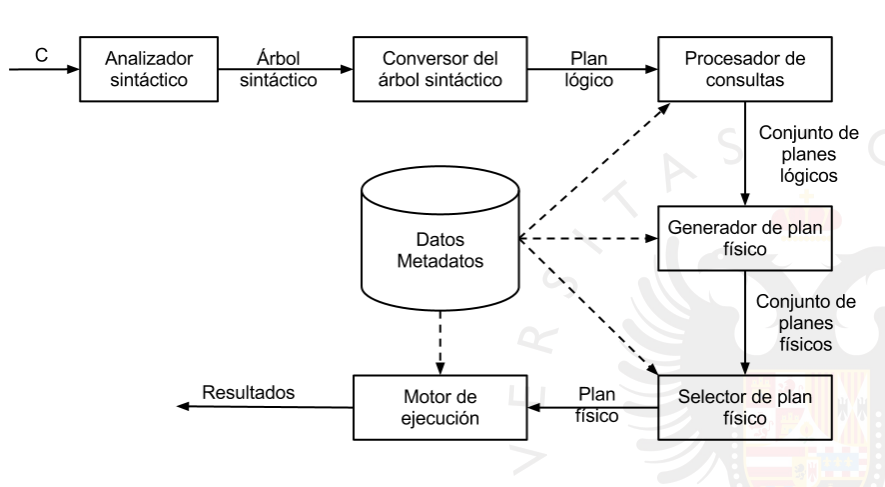
\includegraphics[scale=0.4]{img/1.png}
  \caption{Esquema general de optimización de una consulta}
\end{figure}

\section{Transformación de consultas}

Para transformar la consulta usamos un \textbf{árbol de expresión algebraica} o expresión AR llamado \textbf{plan lógico}. Las hojas de este árbol son las relaciones, los nodos intermedios los operadores y el enlace entre ellos el orden de aplicación.

\begin{example}
El árbol sintáctico $c$ para la siguiente consulta sería:
\begin{lstlisting}[ language=SQL,
                    deletekeywords={IDENTITY},
                    deletekeywords={[2]INT},
                    morekeywords={clustered},
                    framesep=8pt,
                    xleftmargin=40pt,
                    framexleftmargin=40pt,
                    frame=tb,
                    framerule=0pt ]
  SELECT alumno.DNI, alumno.nombre, alumno.calificacion 
  FROM alumno, matricula 
  WHERE alumno.DNI = matricula.DNI 
  AND codigo= "FBD";
\end{lstlisting}
\begin{figure}[H]
  \center
  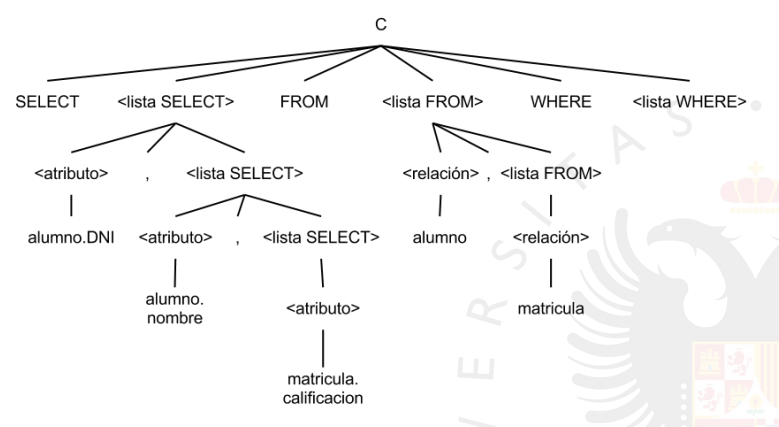
\includegraphics[scale=0.4]{img/2.png}
\end{figure}
Vemos que $<$lista WHERE$>$ no está desarrollado, dos posibles árboles de expresión serían:
\begin{figure}[H]
\centering
\begin{subfigure}{.5\textwidth}
  \centering
  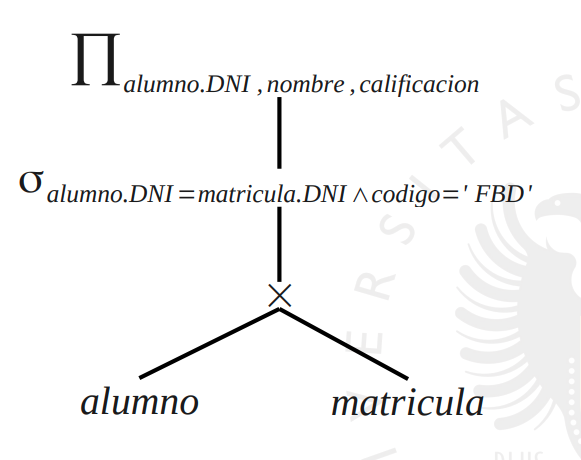
\includegraphics[scale=0.4]{img/3.png}
\end{subfigure}%
\begin{subfigure}{.5\textwidth}
  \centering
  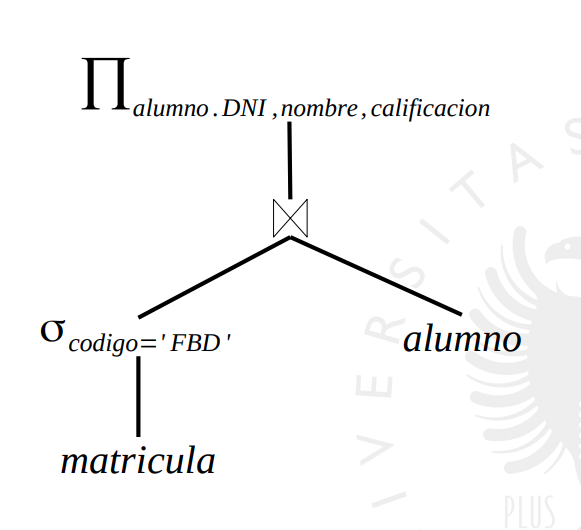
\includegraphics[scale=0.4]{img/4.png}
\end{subfigure}
\end{figure}
\end{example}
Vemos que los dos árboles nos dan un resultado correcto, pero el primero es más costoso de calcular que el segundo. Ahí está la ventaja de estos árboles, mediante una serie de reglas podemos simplicar, eliminar redundancias, etc, para hacer más eficiente una consulta. Algunas de esas reglas son:
\begin{itemize}
\item Conmutatividad de producto, reunión, unión e intersección.
\item Asociatidividad de producto, reunión y unión.
\item Movimiento de selección.
\item Movimiento de proyección.
\item Producto cartesiano.
\end{itemize}
\end{example}

\section{Estrategias para la optimización}
Tenemos varias expresiones equivalentes que difieren en el número de parámetros (tamaño de resultados intermedios, número de tuplas de las relaciones intermedia, etc). El problema es evaluar el coste de cada una, que a su vez también tiene un coste. En general, con $n$ relaciones hay muchas posibilidades:
\[
\frac{(2n-2)!}{(n-1)!}
\]
Un optimizador debe generar un conjunto de planes lo suficientemente amplio para contener el óptimo y lo suficientemente pequeño como para que valga la pena evaluar las posibilidades. Para ello, tenemos varias opciones:
\begin{itemize}
\item Generar un plan según alguna heurística que no es óptimo pero es bueno.
\item Generar todos los planos lógicos posibles, pero sólo funciona para dos relaciones como mucho y crece exponencialmente con la complejidad de la consulta.
\item Una solución mixta: generar un plan seestimargún una heurística y varios planes posibles a partir de él para poder elegir.
\end{itemize}
Cada plan lógico (lo que hay que hacer) genera uno o varios planes físicos (cómo hacerlo), y cada uno incluye:
\begin{itemize}
\item información estadística de datos
\item existencia de índices
\item por cada operador del plan, un algoritmo para aplicarlo
\item los algoritmos de ordenación necesarios
\end{itemize}
Al tener varios planes distintos, necesitamos alguna forma de determinar cuál escoger. Para ello, usamos la estimación de costes. Ejecutar el plan para ver su coste, no es eficiente, obviamente. Además, al principio del plan los datos sobre las relaciones están en el catálogo y conforme avanza la evaluación, dependen de relaciones intermedias y es necesario hacer estimaciones a partir de estadísticas de los datos básicos.

El sistema proporciona algunas estadísticas sobre los datos para ayudarnos a hacer estas estimaciones:

Para una relación ($R$):
\begin{itemize}
\item $N(R)$: número de tuplas de $R$.
\item $L(R)$: longitud en bytes de las tuplas de $R$.
\item $Bfr(R)$: factor de bloqueo de la relación.
\item $B(R)$: número de bloques de la relación $R$.
\end{itemize}
Para un atributo:
\begin{itemize}
\item $V(R,atr):$ número de valores distintos.
\item $nl(R,atr):$ si hay índice sobre el atributo, cuántos niveles tiene un índice multinivel o un B-árbol.
\end{itemize}
Para el sistema:
\begin{itemize}
\item $T(B)$: es el tamaño del bloque en bytes.
\item $C$ es el tamaño de la cabecera del bloque en bytes.
\end{itemize}

\subsection{Tamaño de una proyección}

Dada una relación $R$, la proyección sobre un subconjunto $X$ tendría un tamaño:
\[
L(X)=\sum_{atr_i\in K}size(atr_i)
\]
donde $K$ es el conjunto de atributos del registro. $L$ es la longitud de un registro.
\[
Bfr(X)=\left\lfloor\frac{T(B)-C}{L(X)}\right\rfloor
\]
\[
B(X)=\left\lceil\frac{N(X)}{Bfr(X)}\right\rceil
\]
\begin{example}
Sea la relación $R(a,b,c)$ con $a$ y $b$ enteros ($2B$) y $c$ una cadena de 256 caracteres ($256B$), la cabecera ocupa $16B$ ($C$) y el bloque tiene un tamaño de $T(B)=2048B$. $R$ tiene 1000 registros, es decir $N(R)=1000$.

Calculamos la longitud del registro:
\[
L(R)=2B+2B+256B=260B
\]
Calculamos el factor de bloqueo de esta relación:
\[
Bfr(R)=\left\lfloor\frac{T(B)-C}{L(R)}\right\rfloor=\left\lfloor\frac{2048B-16B}{260B}\right\rfloor=7
\]
Ahora ya podemos calcular el número de bloques de la relación:
\[
B(R)=\left\lceil\frac{N(R)}{Bfr(R)}\right\rceil=\left\lceil\frac{1000}{7}\right\rceil=143
\]
Pero esto es solo para la relación, no para el subconjunto $X$ resultante de la proyección. ¿Cuánto ocupa entonces el resultado de $X=\Pi_{a,b}(R)$? Rehacemos los cálculos pero eliminando de los registros todos los atributos que no aparezcan en la selección, es decir, $N(X)=N(R)=1000$ (porque no eliminamos registros, sino atributos) y $L(X)=2B+2B=4B$.
\[
Bfr(X)=\left\lfloor\frac{T(B)-C}{L(X)}\right\rfloor=\left\lfloor\frac{2048B-16B}{4B}\right\rfloor=508
\]
\[
B(R)=\left\lceil\frac{N(X)}{Bfr(X)}\right\rceil=\left\lceil\frac{1000}{508}\right\rceil=2
\]
\end{example}

\subsection{Tamaño de una selección}

Como el tamaño de la selección depende de cuántos valores cumplan las condiciones de la selección, necesitamos suponer que los datos siguen alguna distribución. La más simple es la uniforme, es decir, la probabilidad de que un atributo tome un valor es un valor constante e igual para todos los valores.

Dada una relación $R$, la selección sobre una condición $c$ tendría un tamaño estimado de
\[
N(X)=\alpha N(R)
\]
donde
\[
\alpha = \left\{
\begin{array}{cl}
\frac{1}{V(R,atr)} & \text{ si } \sigma_{atr=valor}\\
\frac{1}{3} & \text{ si }\sigma_{atr<valor}\\
1 & \text{ si }\sigma_{aatr\neq valor}
\end{array}
\right.
\]
Como una operación de selección no elimina ni añade campos, no afecta a la estructura del registro, luego la longitud y el factor de bloqueo son las mismas tras aplicarla:
\[
L(X)=L(R), \espacio Bfr(X)=Bfr(R)
\]
¿Qué pasa para condiciones compuestas?
\begin{enumerate}
\item Si es una condición AND: aplicamos las selecciones en cascada y multiplicamos los factores de selección.
\item Si es una condición OR: sustituimos por una unión de selecciones y la estimación es:
\[
N(R)\left(1\left(1-\frac{n_1}{N(R)}\right)\left(1-\frac{n_2}{N(R)}\right)\right)
\]
\end{enumerate}

\begin{example}
Base de datos:
\begin{itemize}
\item Alumno (DNI, nombre, fec\_nac, ciudad, direccion, tlfno, beca)
\item Asignatura (codigo, nombre, creditos, caracter, curso)
\item Matricula (codigo, DNI, calificacion)
\end{itemize}
Consulta que queremos optimizar:
\begin{lstlisting}[language=sql]
  SELECT alumno.nombre FROM alumno, matricula 
  WHERE alumno.DNI = matricula.DNI 
  AND beca = "N"
  AND calificacion LIKE "SOBRESALIENTE HONOR%";
\end{lstlisting}
Por simplicidad, usamos la notación:
\[
c_1\equiv \sigma_{beca=N}(Alumnos), \espacio c_2\equiv \sigma_{calificacion=SOBRESALIENTEHONOR}(Matriculas)
\]
Tenemos los siguientes datos de la BD:
\begin{center}
\begin{tabular}{|c|c|c|c|c|}
\hline 
Relación & NTuplas & Bfr & V(Alumnos, Beca) & V(Matrículas, calificacion) \\ 
\hline 
Alumno & 500 & 5 & 2 &   \\ 
\hline 
Matricula & 5000 & 10  &   & 6 \\ 
\hline 
\end{tabular}
\end{center}
Al haber dos valores distintos para Beca, podemos suponer que la mitad tienen beca y la otra mitad no tienen. Luego el número de registros del resultado en $c_1$ sería 250.
\[
N(X)=\frac{1}{V(R,atr)}N(R)=\frac{1}{2}500=250
\]
El factor de bloqueo de $c_1$ es el mismo que el de Alumnos, luego hacen falta 50 bloques para el resultado de $c_1$:
\[
B(R)=\left\lceil\frac{N(X)}{Bfr(X)}\right\rceil=\left\lceil\frac{250}{5}\right\rceil=50
\]
Al haber seis valores distintos para Calificacion, podemos suponer que una sexta parte tienen la calificación buscada. Luego el número de registros del resultado en $c_2$ sería 834:
\[
N(X)=\frac{1}{V(R,atr)}N(R)=\frac{1}{6}5000\approx 250
\]
El factor de bloque de $c_2$ es el mismo que el de Matriculas, luego hacen falta 84 bloques para el resultado de $c_2$:
\[
B(R)=\left\lceil\frac{N(X)}{Bfr(X)}\right\rceil=\left\lceil\frac{834}{10}\right\rceil=84
\]
\end{example}
\subsection{Tamaño de un producto cartesiano}
Este es el más facil de todo, el factor de bloqueo y el número de bloques no cambia, solo el número de registros y la longitud:
Dada una relación $R$, la proyección sobre un subconjunto $X$ tendría un tamaño. Siendo $R$ y $S$ dos relaciones:
\[
N(X)=N(R)N(S)
\]
\[
L(X)=N(R)+N(S)
\]
\[
Bfr(X)=\left\lfloor\frac{T(B)-C}{L(X)}\right\rfloor
\]
\[
B(X)=\left\lceil\frac{N(X)}{Bfr(X)}\right\rceil
\]
\subsection{Tamaño de una reunión natural}
\[
L(X)=L(R)+L(S)-size(b)
\]
donde $b$ es el atributo usado en la reunión natural.

La estimación de $N(X)$ es más compleja y solo se puede hacer si se supone que p ara uno de los atributos de uno de los operandos no se pierde ningún valor al reunir (si había seis valores antes de reunir, hay seis valores después de reunir):
\[
V(R,a)=V(R\;\;JOIN\;\; S,a)
\]
Si la intersección tiene un atributo común, $b$, que toma los mismos malores en ambas tablas:
\[
V(R,b)=V(S,b)
\]
\[
N(X)=\frac{N(R)N(S)}{V(R,b)}=\frac{N(R)N(S)}{V(S,b)}
\]
Si la intersección tiene un atributo en común $b$ y la tabla $S$ hace referencia a la tabla $R$:
\[
V(R,b)\geq V(S,b)
\]
\[
N(X)=\frac{N(R)N(S)}{V(R,b)}
\]
Si la intersección tiene un atributo en común $b$ y la tabla $R$ hace referencia a la tabla $S$:
\[
V(R,b)\leq V(S,b)
\]
\[
N(X)=\frac{N(R)N(S)}{V(S,b)}
\]
Y en general, para que sea más fácil de recordar:
\[
N(X)=\frac{N(R)N(S)}{\max\{V(R,b)V(S,b)\}}
\]
El factor de bloqueo y el número de bloques sigue siendo el mismo:
\[
Bfr(X)=\left\lfloor\frac{T(B)-C}{L(X)}\right\rfloor
\]
\[
B(X)=\left\lceil\frac{N(X)}{Bfr(X)}\right\rceil
\]
\begin{example}
Supongamos la consulta:
\[
R \espacio JOIN \espacio S \espacio JOIN \espacio T
\]
\begin{center}
\begin{tabular}{|c|c|c|}
\hline 
R(a,b) & S(b,c) & T(c,d) \\ 
\hline 
N(R)=5000 & N(S)=3000 & N(T)=1000 \\ 
\hline 
V(R,a)=200 &   &   \\ 
\hline 
V(R,b)=500 & V(S,b)=400 &   \\ 
\hline 
  & V(S,c)=500 & V(T,c)=100 \\ 
\hline 
  &   & V(T,d)=20 \\ 
\hline 
\end{tabular} 
\end{center}
Número de registros:
\begin{figure}[H]
  \center
  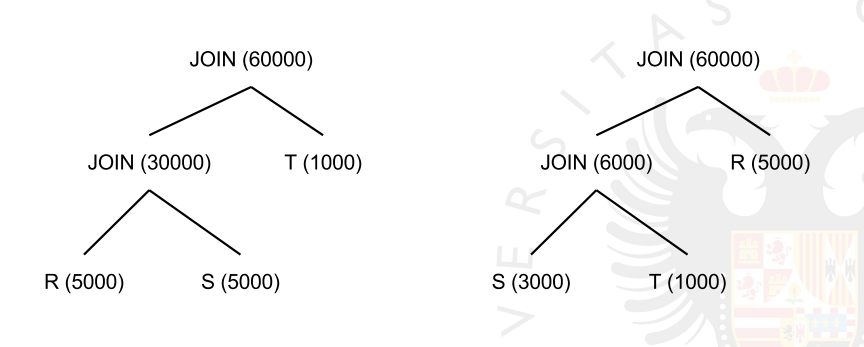
\includegraphics[scale=0.4]{img/7.png}
\end{figure}
Cuidado que hay una errata en el árbol de la izquierda, en el número de registros de $S$, debería ser 3000.
\end{example}
\subsection{¿Cómo trabajan los optimizadores?}
Los SGBD aplican heurísticas de transformación de consultas que, en general, mejoran la eficiencia:
\begin{itemize}
\item Selección lo antes posible.
\item Combinar producto cartesiano y selección en operaciones de reunión.
\item Aplicar la asociatividad para reordenar los nodos hoja de un árbol para realizar las operaciones más restrictivas lo antes posible (lo más a la izquierda y abajo).
\item Proyecciones donde sea posible.
\end{itemize}
 
\chapter{Organización de los datos en un SGBD Relacional}


\begin{figure}[H]
  \center
  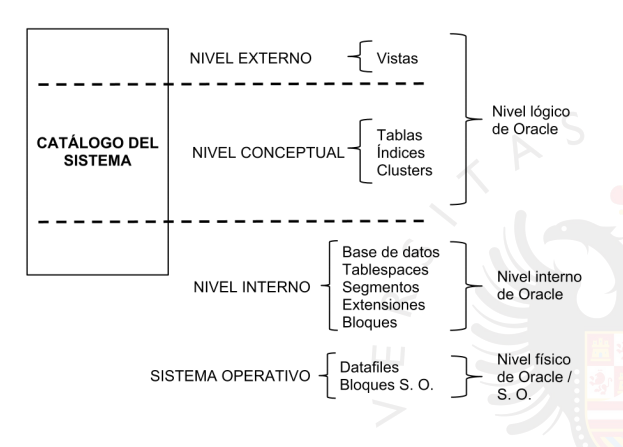
\includegraphics[scale=0.4]{img/8.png}
  \caption{De qué vamos a hablar}
\end{figure}

\section{Catálogo}

En un modelo relacional, toda la información que hay dentro del sistema se almacena en estructuras relacionales, es decir, se almacena información sobre las tablas, en una tabla. Desde esa perspectiva, llamamos \textbf{diccionario de datos} o el \textbf{catálogo} al conjunto de estructuras para almacenar información sobre los datos. Esos datos sobre los datos, se llaman normalmente \textbf{metadatos}.

El catálogo de compone de una serie de objetos entre los que se encuentran:
\begin{itemize}
\item Tablas (atributos, tipos de datos, restricciones, propietario, etc)
\item Vistas (nombre, consulta asociada, propietario, etc)
\item Índices (nombre, tabla, atributos, tipo, propietario, etc)
\item $\cdots$
\end{itemize}
Pero no solo eso, también contiene:
\begin{itemize}
\item Espacio y estructuras de nivel interno
\item Integridad de objetos
\item Usuarios
\item Privilegios y roles
\item Información para auditoría
\item Información sobre la BD (tablespaces, datafiles, etc).
\end{itemize}

Esto significa que el catálogo almacena información sobre \textbf{todos} los niveles de la base datos. ¿Cómo se organiza toda esta información? Como son tablas e índices, se consultan y se manejan como las estructuras de datos estudiadas en los dos capítulos anteriores. Los objetos se almacenan en un tablespace llamado \textbf{SYSTEM}. La información se almacena en:
\begin{itemize}
\item Tablas: denominadas tablas base, sólo accesibles al SGBD y el usuario \textit{sys}, aunque no se recomienda accederlas directamente. El usuario \textit{sys} tiene acceso a ellas porque necesita crearlas al principio de la base de datos. Para consultarlas, se recomienda el uso del siguiente punto.
\item Vistas: sirven para el acceso simple, selectivo y personalizado de la infromación de las tablas base y están accesibles a cualquier usuario (dependiendo de sus permisos).
\end{itemize}

En la organización del catálogo, los nombres de los objetos son importantes:
\begin{itemize}
\item Si comienza por \textbf{USER\_...}: determina que la vista contiene información sobre los objetos del usuario que ejecuta la consulta.
\item Si comienza por \textbf{ALL\_...}: determina que la vista contiene información sobre todos los objetos \textbf{accesibles} para el usuario que ejecuta la consulta (incluya le información de \textit{USER\_...}
\item Si comienza por \textbf{DBA\_...}: determina que la vista consulta la tabla de catálogo tal y como está almacenada (solo el usuario sys y otros con permiso pueden hacerlo).
\end{itemize}

Mantener toda esta estructura sobre la información de la base de datos tiene varias utilidades:
\begin{itemize}
\item Organizar la información de la manera más eficiente posible, y dado que la hemos diseñado con una estructura que permite almacenar información de los usuarios de forma eficiente, ¿por qué no usar esa misma estructura para almecenar la información del sistema?
\item Al tener la información organizada, es mucho más sencillo mantenerla actualizada. Basicamente, todas las operaciones que realizamos sobre el sistema tienen un efecto sobre el catálogo que se actualiza de forma rápida.
\item Además, tener la información almacenada permite conocer mucha información  sobre los tres niveles de la base de datos (externo, conceptual y físico). 
\end{itemize}

\begin{example}
Supongamos la siguiente sentencia sql:
\begin{lstlisting}[ language=SQL,
                    deletekeywords={IDENTITY},
                    deletekeywords={[2]INT},
                    morekeywords={clustered},
                    framesep=8pt,
                    xleftmargin=40pt,
                    framexleftmargin=40pt,
                    frame=tb,
                    framerule=0pt ]
CREATE TABLE CARD (
    CARDID VARCHAR2(20) CONSTRAINT CARD_CARDID_PK PRIMARY KEY,
    CARDNAME VARCHAR2(30) CONSTRAINT CARD_CARNAME_NOTNULL NOT NULL,
    ACCOUNTING VARCHAR2(20)
      CONSTRAINT CARD_ACCOUNTNO_NOTNULL NOT NULL,
      CONSTRAINT CARD_ACCOUNTNO_FK REFERENCES ACCOUNT,
	EXPDATE DATE CONSTRAINT CARD_EXPDATE_NOTNULL NOT NULL,
	DAYLYLIMIT NUMBER(4)
	  CONSTRAINT CARD_DAILYLIMIT_NOTNULL NOT NULL
	  CONSTRAINT CARD_DAILYLIMIT_POSSITIVE CHECK DAILYLIMIT>=0,
	LASTLIMIT NUMBER(6,2)
	  CONSTRAINT CARD_LASTLIMIT_NOTNULL NOT NULL
	  CONSTRAINT CARD_LASTLIMIT_POSSITIVE CHECK LASTLIMIT >=0
	  AND
	  CONSTRAINT CARD_LAST_LIMIT_LESSTHANDAILY
	    CHECK LASTLIMIT <= DAILYLIMIT
);
\end{lstlisting}

Lo primero que se crea es el objeto \textit{CARD} (linea 1). Hay que tener en cuenta que toda tabla de la BD, antes de ser una tabla, es un objeto, es decir, primero tenemos que almacenar información sobre el objeto en sí, y después almacenamos información del objeto visto como tabla. Lo que significa que, después de ejecutar la línea 1, podemos consultar información sobre este objeto en dos tablas diferentes:
\begin{itemize}
\item Vista \textit{USER\_OBJECTS}: que nos dará información de la tabla vista como un objeto.
\item Vista \textit{USER\_TABLES}: que nos dará información de la tabla vista como tabla. 
\end{itemize}
Luego nos encontramos una seria de columnas o atributos (líneas 2,3,4,7,8 y 11) sobre los que también se va a almacenar información. Esta información se va a 
guardar en \textit{USER\_TAB\_COLUMNS}. Sin embargo, como para cada una de las columnas (o atributos) podemos poner una serie de restricciones, incluso más de una, eso nos impide que podamos guardar la información de las restricciones en la misma tabla que guardamos la información de la columna. La información sobre las restricciones se va a guardar en la vista \textit{USER\_TAB\_CONSTRAINTS}.
\end{example}

\section{Estructura interna}

Hablemos ahora de los elementos de la estructura interna de la BD. Lo habitual, es que exista un fichero conteniéndolo 'todo', es decir, ficheros muy grandes con mucha información. De forma que si en un fichero metemos información sobre muchos usuarios y habitualmente los usurios consultan su propia información, es interesante que la información de un usuario esté cercana entre sí. Es decir, organizamos la información del fichero en bloques de forma eficiente para la consulta. Recordemos que a nivel del SO y del sistema de ficheros solo hay bloques y ficheros, pero al nivel físico de Oracle, hay: tablespaces, segmentos, extensiones y bloques. Esos elementos siguen presentan la siguiente jerarquía:

\begin{figure}[H]
  \center
  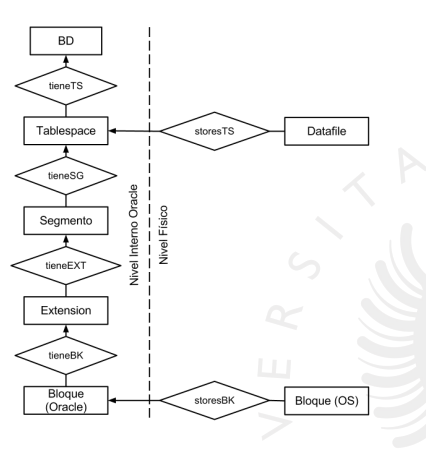
\includegraphics[scale=0.5]{img/9.png}
\end{figure}

Esa imagen que leerla como: la BD tiene \textit{tablespaces} (TS), que se repsentan en el nivel físico mediante \textit{datafiles}. Los \textit{tablespaces} además contienen \textit{segmentos}, y cada segmento almacena una serie \textit{extensiones}, que a su vez tienen \textit{bloques de Oracle} (no del SO). Por último, los bloques de Oracle son almacenados usando bloques del SO.

\subsection{Tablespaces}
\begin{lstlisting}[ language=SQL,
                    deletekeywords={IDENTITY},
                    deletekeywords={[2]INT},
                    morekeywords={clustered},
                    framesep=8pt,
                    xleftmargin=40pt,
                    framexleftmargin=40pt,
                    frame=tb,
                    framerule=0pt ]
CREATE TABLESPACE users DATAFILE "c:\oracle\oradata\users01.dbf" SIZE 20M;
\end{lstlisting}
\begin{figure}[H]
  \center
  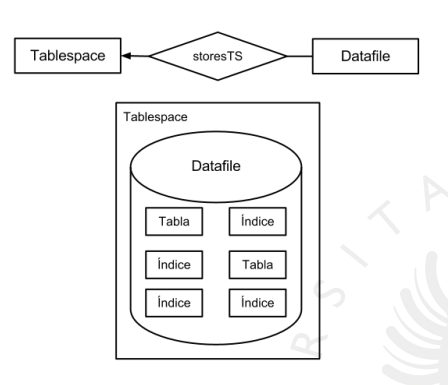
\includegraphics[scale=0.4]{img/10.png}
\end{figure}

Un tablespace se compone de una serie de datafiles, esto quiere decir que cuando se crea uno, hay que especificarle al menos un datafile que se creará dentro de los directorios del SGBD para manejarlo.

Puede darse el caso de que la información dentro de ese tablespace crezca tanto que se sature. En ese caso, lo único que tenemos que hacer es añadirle otro datafile más:

\begin{lstlisting}[ language=SQL,
                    deletekeywords={IDENTITY},
                    deletekeywords={[2]INT},
                    morekeywords={clustered},
                    framesep=8pt,
                    xleftmargin=40pt,
                    framexleftmargin=40pt,
                    frame=tb,
                    framerule=0pt ]
ALTER TABLESPACE users ADD DATAFILE "c:\oracle\oradata\users02.dbf" SIZE 20M;
\end{lstlisting}
\begin{figure}[H]
  \center
  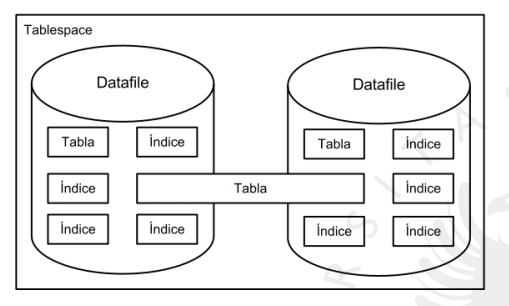
\includegraphics[scale=0.4]{img/11.png}
\end{figure}

De hecho, el SGBD puede repartir la información de los objetos entre los dos datafiles sin ningún problema. Esto implica que un objeto no tiene por qué estar contenido en un único datafile, como vemos en el dibujo, el objeto 'Tabla', está contenido en ambos.

Además, también podemos redimensionar un datafile existente:

\begin{figure}[H]
  \center
  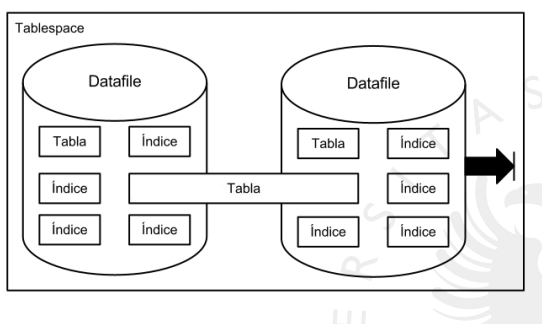
\includegraphics[scale=0.4]{img/12.png}
\end{figure}
\begin{lstlisting}[ language=SQL,
                    deletekeywords={IDENTITY},
                    deletekeywords={[2]INT},
                    morekeywords={clustered},
                    framesep=8pt,
                    xleftmargin=40pt,
                    framexleftmargin=40pt,
                    frame=tb,
                    framerule=0pt ]
ALTER DATABASE DATAFILE "c:\oracle\oradata\users02.dbf" RESIZE 15M;
\end{lstlisting}

Incluso se puede hacer para que el datafile se extienda de forma automática (el uso de \textit{MAXSIZE} se puede omitir, pero es recomendable).

\begin{figure}[H]
  \center
  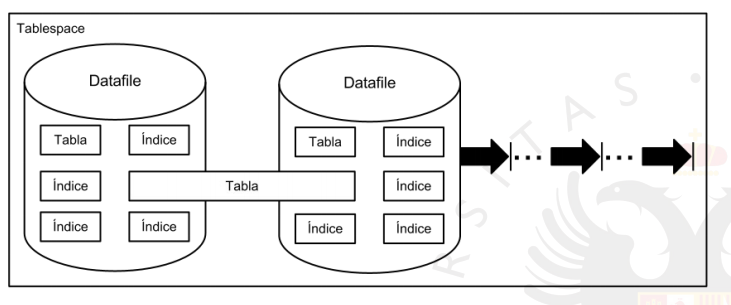
\includegraphics[scale=0.4]{img/13.png}
\end{figure}
\begin{lstlisting}[ language=SQL,
                    deletekeywords={IDENTITY},
                    deletekeywords={[2]INT},
                    morekeywords={clustered},
                    framesep=8pt,
                    xleftmargin=40pt,
                    framexleftmargin=40pt,
                    frame=tb,
                    framerule=0pt ]
ALTER DATABASE DATAFILE "c:\oracle\oradata\users02.dbf" AUTOEXTEND ON NEXT 15M MAXSIZE 100M;
\end{lstlisting}

\subsection{Extensiones, segmentos y bloques}

Internamente, los datafiles almacenan bloques, sin embargo, la forma de estructurar esos bloques no es aleaotria ya que queremos evitar desplazamientos muy largos dentro del disco para poder encontrar rápidamente datos relacionados entre sí. Esa estructura se divide en dos niveles: \textbf{segmentos} y \textbf{extensiones}, de forma que un segmento contiene una serie de extensiones y una extensión contiene una serie de bloques.

Cada vez que se crea una tabla, se crea un segmento que contiene una extensión que contiene un bloque. Es decir, aunque la tabla esté vacía, ocupa espacio (ese bloque). Las extensiones dentro de un segmento se enganchan con punteros y pueden ser de distintos tamaños. Cada extensión contiene un conjunto de bloques. Cuando le extensión se completa, se genera otra extensión encadenada al segmento.

Como al crear el segmento, estamos reservando varios bloques para ese segmento (que no usándolos, ojo) podemos llegar al caso de tener todo el datafile lleno de segmentos, pero con muchos bloques sin usar. ¿Qué pasa si necesitamos crear otro segmento? Se coge un segmento ya existente y se dividen dos si es posible. Luego los segmentos no tienen por qué tener el mismo tamaño.

\begin{figure}[H]
  \center
  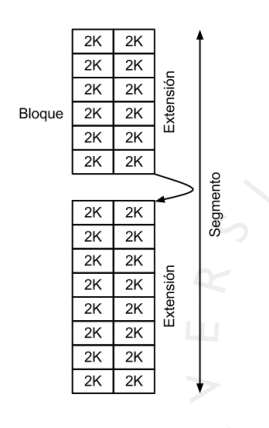
\includegraphics[scale=0.4]{img/14.png}
  \caption{Ejemplo en disco}
\end{figure}

Fijaros que ahí el tamño de las extensiones tampoco es el mismo. ¿Qué tipos de segmentos hay?
\begin{itemize}
\item de datos: tablas
\item de índice: índices
\item temporales: resultados intermedios de \textit{order by}, \textit{group by}, etc. Sobre estos segmentos no hay que almacenar mucha información por eso, porque son temporales y van a desaparecer.
\item de rollback: valores antigusos de datos en \textit{update}. Relacionados con el \textit{redo}, para poder hacer rollback de algunos cambios hechos.
\end{itemize}

Veamos la estructura de un bloque de Oracle:
\begin{itemize}
\item Cabecera: dirección del bloque y tipo de segmento al que está relacionado.
\item Directorio de las tablas que tienen tuplas en el bloque. Cuidado, porque teóricamente lo que hemos visto son los bloques homogéneos, es decir, aquellos bloques que contienen registros de una sola tabla, pero también se pueden contener registros sobre varias tablas en un mismo bloque.
\item Directorio de tuplas del bloque, incluida la dirección. Bastante útil para saltarse tuplas entera (conociendo el offset).
\item Zona de datos donde se almacenan registros. 
\item Espacio libre.
\end{itemize}

\section{Estructura lógica}

El conjunto de objetos de un usuario se denomina \textbf{esquema} y está compuesto por estructuras lógicas como:
\begin{itemize}
\item tablas, vistas, índices, clústers,
\item procedimientos, funciones, paquetes,
\item desparadores, etc.
\end{itemize}
Cada usario tienen un esquema asociado, que tiene el mismo nombre que el usuario al que está relacionado. 

Describamos ahora cada uno de los objetos que puede haber en los esquemas:
\begin{itemize}
\item Tabla: es una estructura lógica con columnas (atributos, identificados por nombre) y filas (tuplas, identificadas por contenido). Al crear una tabla, se crea un segmento con una extensión, y se adjudica a un tablespace por defecto salvo que se especifiquen. Si una fila no cabe en un bloque se genera otro bloque en la extensión, enlazado al anterior, y la tupla se parte.

Cada fila tiene una cabecera con información de cada fragmento, apuntadores, columnas en cada parte, tamaños, etc. Una fila tiene un \textit{rowid} único e invariable. Algunos sistemas admiten el tipo tabla como tipo para una columna.

\begin{example}
Así se crea una tabla asignada al tablespace \textit{users}:
\begin{lstlisting}[ language=SQL,
                    deletekeywords={IDENTITY},
                    deletekeywords={[2]INT},
                    morekeywords={clustered},
                    framesep=8pt,
                    xleftmargin=40pt,
                    framexleftmargin=40pt,
                    frame=tb,
                    framerule=0pt ]
CREATE TABLE CARD ( ... ) TABLESPACE users;
\end{lstlisting}
Recordemos que cada vez que creamos un usuario, se le asigna un tablespace por defecto. Tambíen podemos especificar el tamaño inicial de la extensión ($100K$), el de las siguientes ($100K$) y el número de extensiones máximo que se crearan en el segmento (10):
\begin{lstlisting}[ language=SQL,
                    deletekeywords={IDENTITY},
                    deletekeywords={[2]INT},
                    morekeywords={clustered},
                    framesep=8pt,
                    xleftmargin=40pt,
                    framexleftmargin=40pt,
                    frame=tb,
                    framerule=0pt ]
CREATE TABLE CARD ( ... ) TABLESPACE users 
  STORAGE (INITIAL 100K NEXT 100K MAXEXTENTS 10);
\end{lstlisting}
También podemos eliminar la tabla:
\begin{lstlisting}[ language=SQL,
                    deletekeywords={IDENTITY},
                    deletekeywords={[2]INT},
                    morekeywords={clustered},
                    framesep=8pt,
                    xleftmargin=40pt,
                    framexleftmargin=40pt,
                    frame=tb,
                    framerule=0pt ]
DROP TABLE CARD;
\end{lstlisting}
\end{example}
\item Vista: presentación de datos procedentes de una o más tablas o vistas. Es como guardar una consulta. Se crean mediante el comando \textit{CREATE VIEW}. Para consultar las vistas, se consulta la vista \textit{DBA\_VIEWS}. Básicamente consiste en asignar un nombre a una consulta.

Generalmente, no son actualizables, salvo que se cumplan ciertas restricciones:
\begin{itemize}
\item No pueden incluir agrupadores o agregaciones.
\item No puede incluir la cláusula \textit{DISTINCT}.
\item No puede incluir la reunión ni operadores de conjuntos.
\item Todos los atributos con restricción \textit{NOT NULL} (incluida la clave) deben estar en la vista.
\end{itemize}
Se eliminan mediante la cláusula \textit{DROP VIEW}. ¿Para qué  se usa?
\begin{itemize}
\item Seguridad (ocultar tuplas o atributos)
\item Abstraer de la complejidad de la estructuración de los datos.
\item Simplificar comandos.
\item Aislan aplicaciones de los cambios (si lo que contiene la vista no cambia, claro)
\item Para consultas complejas
\item Para consultas complejas que usan muchos recursos (para no tener que construirlas muchas veces).
\end{itemize}
\item Índice: agilizan el acceso pero ocupan espacio. Enlentecen las inserciones y modificaciones. Hay que pensarlo dos veces antes de crearlos. Oracle crea un índice para la clave (no crees otro). Se usan para:
\begin{itemize}
\item Buscar registros por valores específicos (en columnas indexadas)
\item Recorrer una tabla en orden distinto al físico (ORDER BY)
\item Buscar registros en un rango (en columna indexada)
\end{itemize}
La sentencia para crearlos en \textit{CREATE INDEX}. Después de crear la tabla, mejor insertar las tuplas y después crear al índice (para evitar todas las actualizaciones). La indexación típica suele ser un árbol $B^*$ equilibrado, aunque puede usar bitmaps o hash.
\item Índices multiatributo: índices con más de un atributo son útiles cuando se consulta por los valores de esos atributos de manera ordenada o, en caso de consultarse menos, se consultan desde el primero en adelante. Precisan de mantenimiento, luego deberíamos borrarlos si:
\begin{itemize}
\item Ya no sirven
\item No mejoran la eficiencia
\item Hay que cambiar los campos que se indexan
\item Hay que rehacerlo
\end{itemize}
Para borrarlos se usa la sentencia \textit{DROP INDEX}. Dentro del catálogo se pueden consultar en las tablas \textit{DBA\_INDEXES} y \textit{DBA\_IND\_COLUMNS}.
\item Clusters: para el almacenamiento cercano de tablas que comparten campos y a las que se accede de forma conjunta (reunión natural). Si se accede a cada tabla individualmente y de forma frecuente, no es eficiente. Si se modifican frecuentemente las tablas (en tuplas) no es eficiente. Mejoran la reunión natural al reducir los accesos a disco. El campo o campos de reunión natural se almacenan una sola vez (claro ejemplo de bloques heterogéneos). ¿Cómo se crea? Primero se crea con \textit{CREATE CLUSTER}. Luego hay que crear las tablas del cluster:
\begin{lstlisting}[ language=SQL,
                    deletekeywords={IDENTITY},
                    deletekeywords={[2]INT},
                    morekeywords={clustered},
                    framesep=8pt,
                    xleftmargin=40pt,
                    framexleftmargin=40pt,
                    frame=tb,
                    framerule=0pt ]
CREATE TABLE <nombre> (
  ...
) CLUSTER <nombre> (<campos de reunion>);
\end{lstlisting}
Antes de insertar datos, crear el índice sobre los campos del clúster:
\begin{lstlisting}[ language=SQL,
                    deletekeywords={IDENTITY},
                    deletekeywords={[2]INT},
                    morekeywords={clustered},
                    framesep=8pt,
                    xleftmargin=40pt,
                    framexleftmargin=40pt,
                    frame=tb,
                    framerule=0pt ]
CREATE INDEX <nombre> ON CLUSTER <nombre>;
\end{lstlisting}
Puede borrarse con la sentencia \textit{DROP CLUSTER}, pero primero hay que borrar las tablas de dentro, o usar la sentencia \textit{INCLUDING TABLES}. También hay que borrar las llaves externas que las referencian salvo que se incluya la sentencia \textit{CASCADE CONSTRAINTS}. Se puede borrar su índice con \textit{DROP INDEX} pero no se podrá acceder al contenido del clúster si no se reconstruye dicho índice.
\end{itemize}

\end{document}

